\documentclass[12pt]{article}

\usepackage{fancyhdr}
\usepackage{lastpage}
\usepackage{float}
\usepackage{tikz}
\usepackage{amsmath}
\usepackage{pgfplots}
\usepackage{multirow}
\usepackage{caption}
\usepackage{amssymb}
\usepackage{subcaption}
\usepackage{listings}
\usepackage{diagbox}
\usepackage{longtable}
\usetikzlibrary{automata,positioning,arrows}
\usepackage[top=2.2in, left=0.75in,right=0.75in,headsep=1mm,footskip=.5in]{geometry}

\usepackage{array}
\usepackage{multirow}
\usepackage{float}
\usepackage{booktabs}


\usepackage{ifthen}
\newboolean{showsolutions}
\setboolean{showsolutions}{false} % change to show/hide solutions.
\ifthenelse{\boolean{showsolutions}}{%
  % When showing solutions
  \newenvironment{solution}
    {\par\noindent\textbf{\textcolor{blue}{Solution:}}\par}
    {}
}{%
  % When hiding solutions: just ignore content
  \newenvironment{solution}
    {\expandafter\ignorespaces}
    {}
}
\usepackage{xcolor}


\makeatletter
\newcommand\cdotfill{%
    \leavevmode\cleaders\hb@xt@.44em{\hss$.$\hss}\hfill\kern\z@
}
\makeatother

% Custom line background command
\definecolor{lightgray}{gray}{0.95}
\definecolor{white}{gray}{1.0}
\makeatletter
\lst@AddToHook{OnLine}{%
  \ifnum\value{lstnumber}=0\relax\else
    \ifodd\value{lstnumber}
      \color{white}\lst@basicstyle\colorbox{white}{\strut}
    \else
      \color{lightgray}\lst@basicstyle\colorbox{lightgray}{\strut}
    \fi
  \fi
}
\makeatother

\usepackage{algorithm}
\usepackage{algpseudocode}

\pagestyle{fancy}
\let\headrule\empty
\let\footrule\empty
\rhead{\hrule}
\chead{\hrule}
\lhead{\hrule}
\lfoot{CSC\,263\,H1, Fall 2025}
\cfoot{Page \thepage\space of \pageref{LastPage}}
    \rfoot{Quiz 1}

\DeclareMathOperator*{\argmax}{arg\,max}
\DeclareMathOperator*{\argmin}{arg\,min}

\begin{document}

\newcommand{\checkbox}[1][Option]{
  \begin{tikzpicture}[baseline=0]
    \node[draw=black, minimum size = 0.5cm] (s) {};
    \node[right = 0cm of s, align = left]{#1};
  \end{tikzpicture}%
}

\newcommand{\checkboxmath}[1][Option]{
  \begin{tikzpicture}[baseline=0]
    \node[draw=black, minimum size = 0.5cm] (s) {};
    \node[right = 0cm of s, yshift=-1mm, align = left]{#1};
  \end{tikzpicture}%
}

\newcommand{\points}[1][0]{
  {[#1 pts]}
}

\newcommand{\choice}[1][Option]{
  \begin{tikzpicture}[baseline=0]
    \node[circle, draw=black, minimum size = 0.5cm] (s) {};
    \node[right = 0cm of s, yshift=-0.7mm, align = left]{#1};
  \end{tikzpicture}%
}

\newcommand{\tf}{
  \\~\\
  
\begin{tikzpicture}
    \node[circle, draw=black, minimum size = 0.5cm] at (0,0) (t) {};
    \node[right = 0cm of t, yshift=-1mm, align = left]{True};


    \node[circle, draw=black, minimum size = 0.5cm] at (4,0) (f) {};
    \node[right = 0cm of f, yshift=-1mm, align = left]{False};
  \end{tikzpicture}%
}

\newcommand{\numbox}[1][5em]{
  \begin{tabular}{|c|}         \hline \hspace{#1} \\ \\ \\ \hline     \end{tabular}
}

\newcommand{\fractional}[1][]{
  #1 \begin{tabular}{|c|}         \hline \hspace{5em} \\ \\ \\ \hline     \end{tabular} $\Bigg/$ \begin{tabular}{|c|}         \hline \hspace{5em} \\ \\ \\ \hline     \end{tabular}
}

\newcommand{\tableanswer}[1][Title]{
  \begin{tabular}{|l|}         \hline #1 \\ \hspace{5em} \\ \\ \hline     \end{tabular}%
}

\newcommand{\blank}[1][2cm]{
\underline{\hspace{#1}}
}

\newcommand{\infobox}[1][Title]{
  \noindent #1
  \begin{table}[H]
    \begin{tabular}{|c|c|c|c|c|c|c|c|c|c|c|c|c|c|c|c|c|}
      \hline
      \hspace{1.2em}\; & \hspace{1.2em}\; & \hspace{1.2em}\; & \hspace{1.2em}\; & \hspace{1.2em}\; & \hspace{1.2em}\; & \hspace{1.2em}\; & \hspace{1.2em}\; & \hspace{1.2em}\; & \hspace{1.2em}\; & \hspace{1.2em}\; & \hspace{1.2em}\; & \hspace{1.2em}\; & \hspace{1.2em}\; & \hspace{1.2em}\; & \hspace{1.2em}\; & \hspace{1.2em}\; \\
      \hspace{1.2em}\; & \hspace{1.2em}\; & \hspace{1.2em}\; & \hspace{1.2em}\; & \hspace{1.2em}\; & \hspace{1.2em}\; & \hspace{1.2em}\; & \hspace{1.2em}\; & \hspace{1.2em}\; & \hspace{1.2em}\; & \hspace{1.2em}\; & \hspace{1.2em}\; & \hspace{1.2em}\; & \hspace{1.2em}\; & \hspace{1.2em}\; & \hspace{1.2em}\; & \hspace{1.2em}\; \\\hline
    \end{tabular}%
  \end{table}
}

\newcommand{\spacer}[]{
  \vspace{5mm}\\
}

\newcommand{\hspacer}[]{\\
}

\begin{center}\large
  UNIVERSITY OF TORONTO\\
  Faculty of Arts and Science\\[1.75ex]
  Department of Computer Science\\[1.75ex]
  \textbf{Quiz 1} \\
  \textbf{{CSC\,263\,H1}}
\end{center}

\infobox[\textbf{First Name:}]
\infobox[\textbf{Last Name:}]

\noindent \textbf{Student \# (9 or 10 digits):} \begin{table}[H]
    \begin{tabular}{|c|c|c|c|c|c|c|c|c|c|}
      \hline
      \hspace{1.2em}\; & \hspace{1.2em}\; & \hspace{1.2em}\; & \hspace{1.2em}\; & \hspace{1.2em}\; & \hspace{1.2em}\; & \hspace{1.2em}\; & \hspace{1.2em}\; & \hspace{1.2em}\; & \hspace{1.2em}\; \\
      \hspace{1.2em}\; & \hspace{1.2em}\; & \hspace{1.2em}\; & \hspace{1.2em}\; & \hspace{1.2em}\; & \hspace{1.2em}\; & \hspace{1.2em}\; & \hspace{1.2em}\; & \hspace{1.2em}\; & \hspace{1.2em}\;\\\hline
    \end{tabular}%
  \end{table}
\noindent \textbf{UTORid (e.g. \texttt{gummalur}):} \begin{table}[H]
    \begin{tabular}{|c|c|c|c|c|c|c|c|}
      \hline
      \hspace{1.2em}\; & \hspace{1.2em}\; & \hspace{1.2em}\; & \hspace{1.2em}\; & \hspace{1.2em}\; & \hspace{1.2em}\; & \hspace{1.2em}\; & \hspace{1.2em}\; \\
      \hspace{1.2em}\; & \hspace{1.2em}\; & \hspace{1.2em}\; & \hspace{1.2em}\; & \hspace{1.2em}\; & \hspace{1.2em}\; & \hspace{1.2em}\; & \hspace{1.2em}\;\\\hline
    \end{tabular}%
  \end{table}
\noindent \textbf{Duration:}\cdotfill {50 minutes}\\
\textbf{Instructor:}\cdotfill Chandra Gummaluru\\
\textbf{Weight:}\cdotfill 10\% \\
%\textbf{Aids Allowed:}
%\begin{enumerate}
%    \item[(1)] Non-Programmable Calculator 
%\end{enumerate}
\\~\\
\begin{center}
    \textit{Do NOT turn over the page until you are told to do so.}
\end{center}

\clearpage


\lstdefinestyle{mypython}{
    language=Python,
    keywordstyle=\color{blue}\bfseries,
    stringstyle=\color{orange},
    commentstyle=\color{gray}\itshape,
    basicstyle=\ttfamily\normalsize,
    numbers=left,
    numberstyle=\tiny\color{gray},
    stepnumber=1,
    numbersep=5pt,
    xleftmargin=15pt,
    frame=none,
    showstringspaces=false,
    breaklines=true,
    breakatwhitespace=true,
    tabsize=4,
    columns=flexible
}
\lstset{style=mypython} % Apply default style

\begin{document}
\setcounter{chapter}{1}
\MakeScribeTop

\setlength\parindent{0pt}

\subsection*{Question 1.1: Complexity Analysis}
\points[4] Consider the following \texttt{Python} function:
% Here, I modify the existing problem but the main idea is similar. First loop is reversed geometric series (1 + 2 + 4 + ... n = O(n))
% The second loop tests student's knowledge on log complexity.
\begin{lstlisting}[language=Python]
def mystery_function(arr):
    n = len(arr)
    result = 0
    step = n
    while step > 0:
        for i in range(n):
            for j in range(i, n):
                if j < step:
                    result += arr[i] * arr[j]
                else:
                    result -= arr[i] + arr[j]
        step //= 2
    
    return result
\end{lstlisting}
Determine the time complexity of \texttt{mystery\_function} in terms of $n = \texttt{len(arr)}$. Show your work.
\\~\\
The time complexity of \texttt{mystery\_function} is $O\left(\numbox[4cm] \right)$.


\newpage
\subsection*{Question 1.2: Graphs}
Recall that a directed, weighted graph can be defined as $\mathcal{G} = (V, E, \textsf{chl}, \textsf{wgt})$, where $V$ is the set of vertices, $E \subseteq V \times V$ is the set of edges, $\textsf{chl}: V \rightarrow \textsf{pow}(V)$ is the child function, and $\textsf{wgt}: E \rightarrow \mathbb{R}_{+}$ is a weight function.
\\~\\
Consider a graph with 6 vertices labelled \texttt{a}, $\dots$, \texttt{f} as shown below:
\begin{center}
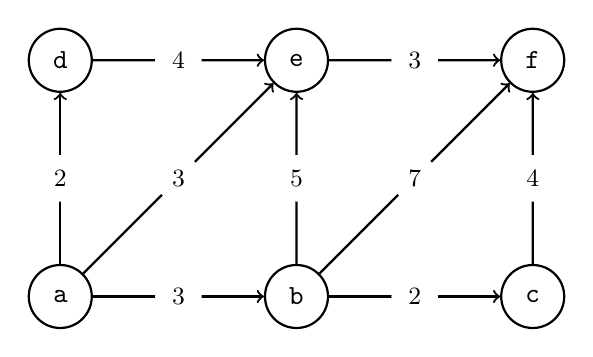
\begin{tikzpicture}[scale=1.2]
\begin{scope}[every node/.style={circle,thick,draw,minimum size=8mm}]
    \node (A) at (0,0) {\texttt{a}};
    \node (B) at (2.5,0) {\texttt{b}};
    \node (C) at (5,0) {\texttt{c}};
    \node (D) at (0,2.5) {\texttt{d}};
    \node (E) at (2.5,2.5) {\texttt{e}};
    \node (F) at (5,2.5) {\texttt{f}};
\end{scope}
\begin{scope}[every node/.style={fill=white,circle,font=\small}, every edge/.style={draw=black, thick}]
    \path [->] (A) edge node {$3$} (B);
    \path [->] (B) edge node {$2$} (C);
    \path [->] (D) edge node {$4$} (E);
    \path [->] (E) edge node {$3$} (F);
    
    \path [->] (A) edge node {$2$} (D);
    \path [->] (B) edge node {$5$} (E);
    \path [->] (C) edge node {$4$} (F);
    
    \path [->] (A) edge node {$3$} (E);
    \path [->] (B) edge node {$7$} (F);
\end{scope}
\end{tikzpicture}
\end{center}
\textbf{Important Note:}\\Since vertices labels are not integers, we will need to use \texttt{Python} dictionaries to store its vertices and edges. You do not need to know the details of how dictionaries work to complete this question.  
For the purpose of this task, you can think of a dictionary as being similar to a list, but instead of using only integer indices (\texttt{0}, \texttt{1}, \texttt{2}, \dots), it allows you to use other types as keys, such as strings.
\\~\\
For example:
\begin{lstlisting}
my_dict = {"chandra-s25": ["helen-pc", "zws-323"], "helen-pc": ["ws-14"]}
print(my_dict["chandra-s25"]) # prints ["helen-pc, router-051797"]
\end{lstlisting}
\clearpage
\begin{enumerate}
    \item \points[3] Consider the following adjacency matrix representation of a graph.
    \begin{lstlisting}[style=mypython]
class Graph:
    def __init__(self, child_matrix):
        # matrix of children and assocaited edge weights, where element ['a']['b'] represents the edge from Vertex a to Vertex b
        self.child_matrix = child_matrix
\end{lstlisting}
    Construct the graph using this representation. In particular, provide the lines of \texttt{Python} code needed to represent the graph. You may not need all the lines.
\begin{lstlisting}[numberblanklines=true, keepspaces=true,showlines=true, numberstyle=\large\ttfamily\color{gray}, lineskip=12pt]















\end{lstlisting}
    \newpage
    \item \points[3] Consider the following adjacency-list implementation of a graph.
      \begin{lstlisting}[style=mypython]
class Vertex:
    def __init__(self):
        # dictionary of child vertices and associated edge weights
        # (vertex_label, weight)
        self.children = {}
        
class Graph:
    def __init__(self, verticies):
        # list of vertices
        self.vertices = vertices
\end{lstlisting}
Construct the graph using this representation. In particular, provide the lines of \texttt{Python} code needed to represent the graph. You may not need all the lines.
\begin{lstlisting}[numberblanklines=true, keepspaces=true,showlines=true, numberstyle=\large\ttfamily\color{gray}, lineskip=12pt]












\end{lstlisting}
\end{enumerate}
\clearpage

\newpage

\subsection*{Question 1.3: Cheapest-Path Algorithms}
\begin{enumerate}
    \item \points[3] What is the time-complexity of Breadth-First Search (BFS) in terms of $V$ and $E$? Explain your answer and state any assumptions.
    \\~\\
The time complexity of BFS is $O\left(\numbox[4cm] \right)$.
\vspace{5cm}

    \item \points[7] Run Cheapest-First Search (CFS) / Uniform Cost Search (UCS) on the graph from Question 1.2, with $v^{(0)} = \texttt{a}$ and $G = \lbrace \texttt{f}\rbrace$. Break ties in alphabetic order. Show the contents of $\mathcal{O}$ during each iteration of the algorithm.
    \\~\\
    Use the following notation to represent a node that contains a path, $p = \langle (\varnothing, v_0),\dots,(v_{k-1},v_k)\rangle$, with cost $c = \textsf{cst}(p)$: $\left(\langle v_0,v_1,v_2,v_3,\dots,v_k\rangle, c\right)$.
    \\~\\
    \textit{Hint}: Initially, $\mathcal{O} \leftarrow \lbrace (\langle\rangle, 0)\rbrace$. You may not need all the rows.

\begin{longtable}{|>{\centering\arraybackslash}m{5cm}|>{\centering\arraybackslash}m{11cm}|}
\hline
Explored Node, $n$ & Open Set, $\mathcal{O}$ (before expansion of $n$) \\
\hline
\endfirsthead

\hline
\textbf{Node, $n$} & \textbf{Open Set, $\mathcal{O}$} \\
\hline
\endhead

\hline
\multicolumn{2}{r}{\small\itshape continued...} \\
\endfoot

\hline
\endlastfoot

\diagbox[width=5.45cm,height=4em]{}{} & \\
\hline
 & \\[3em]
\hline
 & \\[3em]
\hline
 & \\[3em]
\hline
 & \\[3em]
\hline
 & \\[3em]
\hline
 & \\[3em]
\hline
 & \\[3em]
\hline
 & \\[3em]
\hline
 & \\[3em]
\hline
 & \\[3em]
\hline
 & \\[3em]
\hline


\end{longtable}

\end{enumerate}

\clearpage
\newpage
\begin{center}
    \textit{(rough work - this page will not be marked)}
\end{center}
\clearpage

\end{document}